\documentclass{article}
\usepackage{graphicx} % Required for inserting images
\graphicspath{ {./images/} }
\usepackage{mathtools}
\usepackage{amsfonts}
\usepackage{float}

\title{Low-rate Deletion Correcting Codes}
\author{Daniel Noor \& Orel Adivi}
\date{May 2024}

\begin{document}

\maketitle

\begin{abstract}
    We present several ideas for creating deletion-correcting codes with $O(\log(n))$ information bits and comparing them. Our most notable result is a code-generation method, which augments the random generation of codewords to achieve better capabilities than other tested codes.
\end{abstract}

\section{Introduction}
This project deals in \textbf{deletion correcting codes} - codes which allow us to decode the original encoded value despite deletions occurring in the codeword. The exact number of deletions which a code can correct varies from one code to another. These codes can have a variety of applications, for example dealing with loss of packets during network transmissions.
We focus on \textbf{low-rate} deletion correcting codes \cite{dcc_intro}. Low-rate codes have a relatively small amount of information bits compared to redundancy bits.

In our case, the codes have $O(log(n))$ information bits, where $n$ is the number of bits in each codeword. To ensure that there are indeed $O(log(n))$ information bits, we aimed for codes which contain $n$ words. The goal of our project was to create low-rate deletion correcting codes, which can correct as many deletions as possible.

Some of our codes utilized \textbf{Varshamov–Tenengolts codes}. For each $a = 0,1,...,n$ ($n$ is the codeword length), The corresponding Varshamov–Tenengolts (VT) code is defined as follows \cite{VT}:

\[VT_a(n) = \{x \in \mathbb{F}_2^n | \Sigma_{i=1}^n ix \bmod n+1\}\]

\noindent The above definition assumes binary codewords. For q-ary codewords, we define:

\[VT_a(n, q) = \{x \in \mathbb{F}_q^n | \Sigma_{i=1}^n ix \bmod n+1\}\]

\noindent In the following sections, we outline the different codes we developed and their evaluations.


\section{Calculating the Deletion Distance}
The \textbf{deletion distance} between two strings is the minimum number of characters needed to be deleted from both strings in order to get the same string. It is used in the decoding process to match a codeword with deletions to the "intended" original codeword.

We have computed the deletion distance using dynamic programming (DP). Our implementation was based on a DP method to compute the Levenshtein distance between strings \cite{DP}. Levenshtein distance is an expanded version of deletion distance, taking into account insertions and substitutions as well as deletions \cite{Levenshtein}.
Let us briefly explain the idea behind the implementation.

Let $s_1, s_2$ be the two strings between which we want to measure the deletion distance. In our code, we assume that the deletions occur only in $s_1$ (meaning $s_1$ is contained in $s_2$). We first fill out a table of size $len(s_1)+1 \times len(s_2)+1$ with zeros. Then we iterate over both words and fill the cells, each representing a sub-problem. Cell $i,j$ is filled with the deletion distance between $s_1[0:i]$ and $s_2[0:j]$. The value of each cell is computed from previous cells: if $s_1[i]$ is equal to $s_2[j]$ then cell $i, j$ is equal to cell $i-1, j-1$ (since identical bits do not increase the deletion distance). Otherwise, cell $i, j$ is equal to 1 plus the value of cell $i, j-1$. This represents deleting one bit from $s_2$ and computing the resulting deletion distance.

The exact implementation appears in our GitHub repository.


\section{Codes}
Below is a short description of every type of code we have created as part of the project. The implementations of each code appear in our GitHub repository as well.

\subsection{Random Code}

As a baseline, we first create a random code generator. Given a codeword length $n$, the generator creates a code comprised of $n$ random different codewords (created using \texttt{numpy.random.choice}). This code was created mainly to measure how effective other codes are at correcting errors.

\subsection{Greedy Code}

The idea behind the greedy code was to create codewords one by one, such that each new codeword would be as different as possible from each other.

To that end, when creating a new codeword we begin with a random word. Then, we go over all existing codewords. In iteration $i$, if bit $i$ of the new codeword is equal to bit $i$ of the current iteration's codeword, we flip it (turn 0 to 1). If the two bits are different, we instead choose bit $i$ of the new codeword randomly.

A greedy code of 3 words, for example, would be comprised of a random word $w$, $\bar{w}$ and a word sharing half its bits (in expectation) with each of the previous words.

\subsection{Lin-space Code}

This code utilizes the \texttt{numpy.linspace} function. First of all, we include the all-$0$ word and all-$1$ word in the code. Then, for every $l$ in \texttt{numpy.linspace} from 1 to $n/2$ we add the word which alternates between $l$-long sequences of 0's and 1's.

For example, for $l=1$ we get the word $01010101...$ and for $l=n/2$ we get the word $0000...1111$.

We expected that making sure the codewords had as few shared sequences as possible would keep the deletion distances between them high. While this code works better than the previous ones for a smaller number of codewords, it could not be expanded to create a code of $n$ words.

\subsection{Log-space Code}

This code is similar to the previous one. Here, for every $l$ in \texttt{numpy.logspace} from $1$ to $n$ we add the word which alternates between $1$-long sequences of $0$'s and $1$'s.

For a smaller number of codewords, this code works better than the lin-space code but still has the same problem.

\subsection{Repetition Code}

This code is based on the idea of taking all the words of length $m$, which is smaller than the code size $n$, and then duplicating each character $\frac{n}{m}$ times.

For $m = \log(n)$ this yields a code of exactly $n$ words, and we expected this code to be able to correct roughly $\frac{n}{\log(n)}$ deletions. This estimate stemmed from the fact that for each difference between two words of length $\log(n)$, there will be $\frac{n}{\log(n)}$ differences in the corresponding codewords (where "difference" here refers to Hamming distance).

\subsection{VT Repetition Code}

This code is similar to the repetition code, but instead of taking all the words of length $m$ we only take words that belong to VT$_0(m)$. In order to reach $n$ codewords, $m$ needs to be increased. We have experimented with an $m$ value of $\log(n) + \log\log(n)$, which gives a code size slightly larger than $n$. Redundant codewords are removed to reach a code of exactly size $n$.

We reasoned that this idea could improve upon the repetition code, as the words we duplicate to create our codewords are already taken from a code capable of correcting one deletion.

\subsection{N-ary VT Repetition Code}

After implementing the VT repetition code, we tried another variation of the idea.
This code is very similar to the previous one, only instead of taking words that belong to VT$_0(m)$ we take words that belong to VT$_0(m, q)$ and convert them to a binary base. Again, we have chosen an $m$ value of $\log(n) + \log\log(n)$.

\subsection{Random/Greedy Code}

Since the random code seemed to work better than the others, we tried to create another code based on random selection. The original random code was created by generating words one by one and inserting them into the code.

The random/greedy code generates pairs of words instead. After generating a new pair, only the "better" word of the two, that has a larger deletion distance from the existing codewords, will be inserted into the code. Later on, we allowed changing the number of codeword candidates generated in each iteration.


\section{Evaluation}
We have performed several experiments, some comparing entirely different codes and some comparing the same code generation method with modified parameters.

\begin{figure}[H]
    \centering
    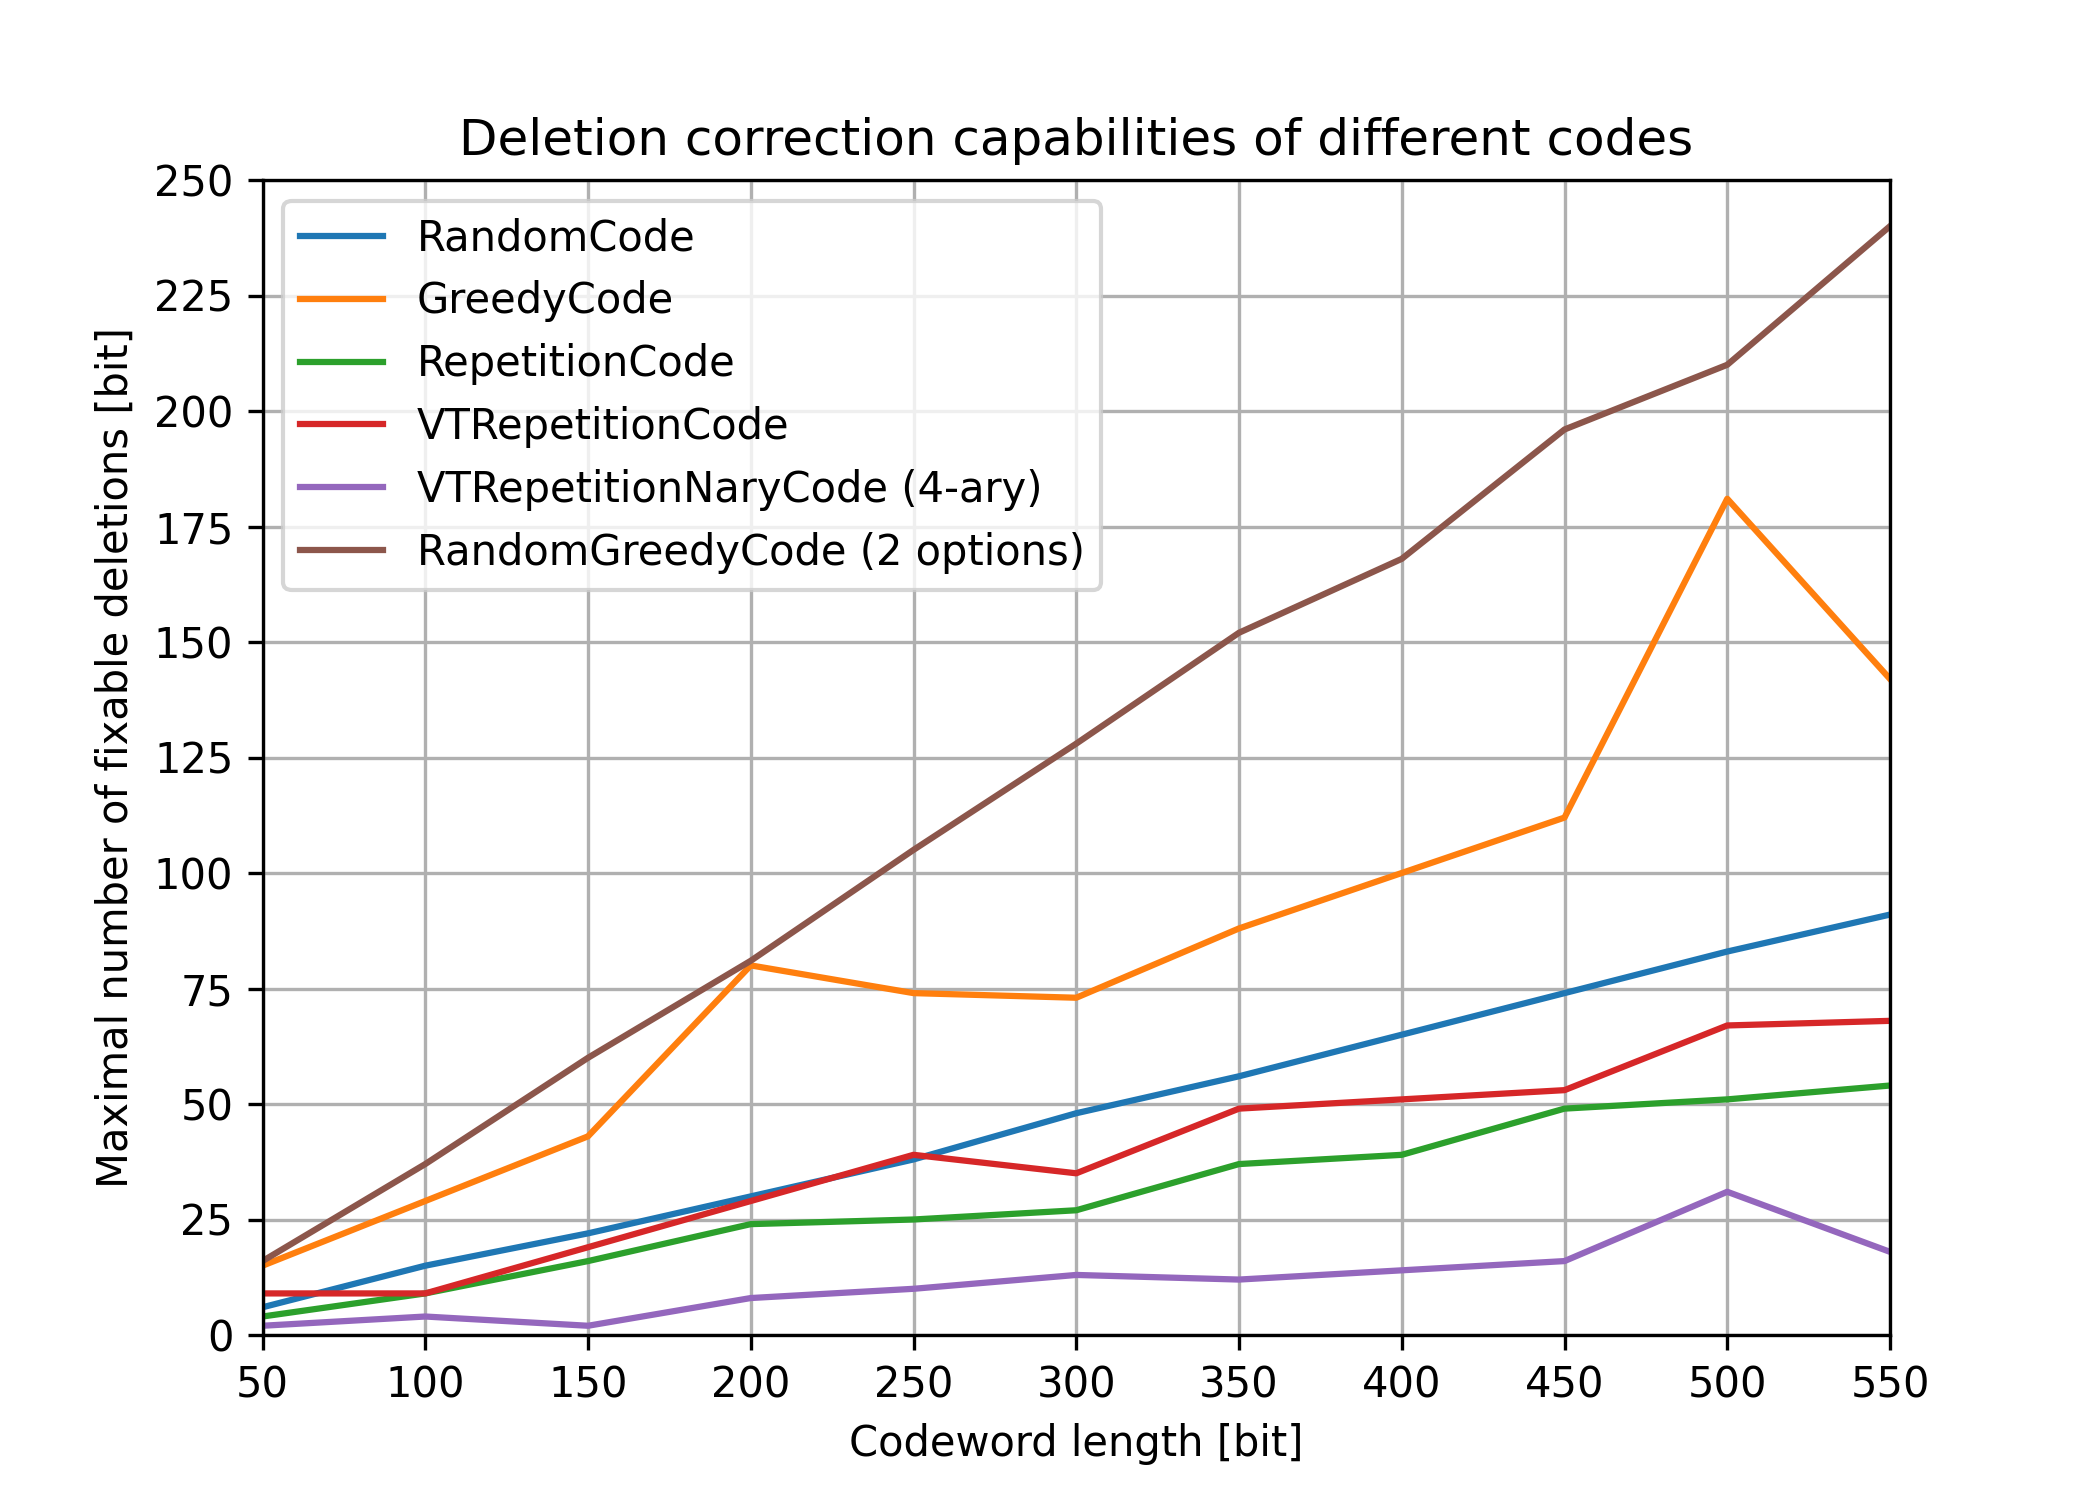
\includegraphics[width=1\textwidth]{artifacts/figure1.png}
    \caption{Comparison between all the valid codes.}
\end{figure}

\noindent In Figure 1, all the codes are represented except for the linspace and logspace codes (as they contain less than $n$ words and therefore cannot be properly compared with the other codes). For the n-ary code, base 4 was used, and for the Random/Greedy Code, 2 codeword candidates were generated in each iteration.

We can see that all three repetition codes perform worse than the randomly generated code, which is our baseline.
The greedy and random/greedy codes both perform better, but surprisingly the random/greedy code pulls ahead. We theorize that this is because the algorithm we use to generate the greedy code is unsophisticated and does not truly select the "best" word in each iteration. However, the random/greedy code generator does select the measurably better word in each iteration, which might explain the results. Overall, it is the most promising code and seems to consistently be able to correct more than twice the number of deletions that the random code can.

\begin{figure}[H]
    \centering
    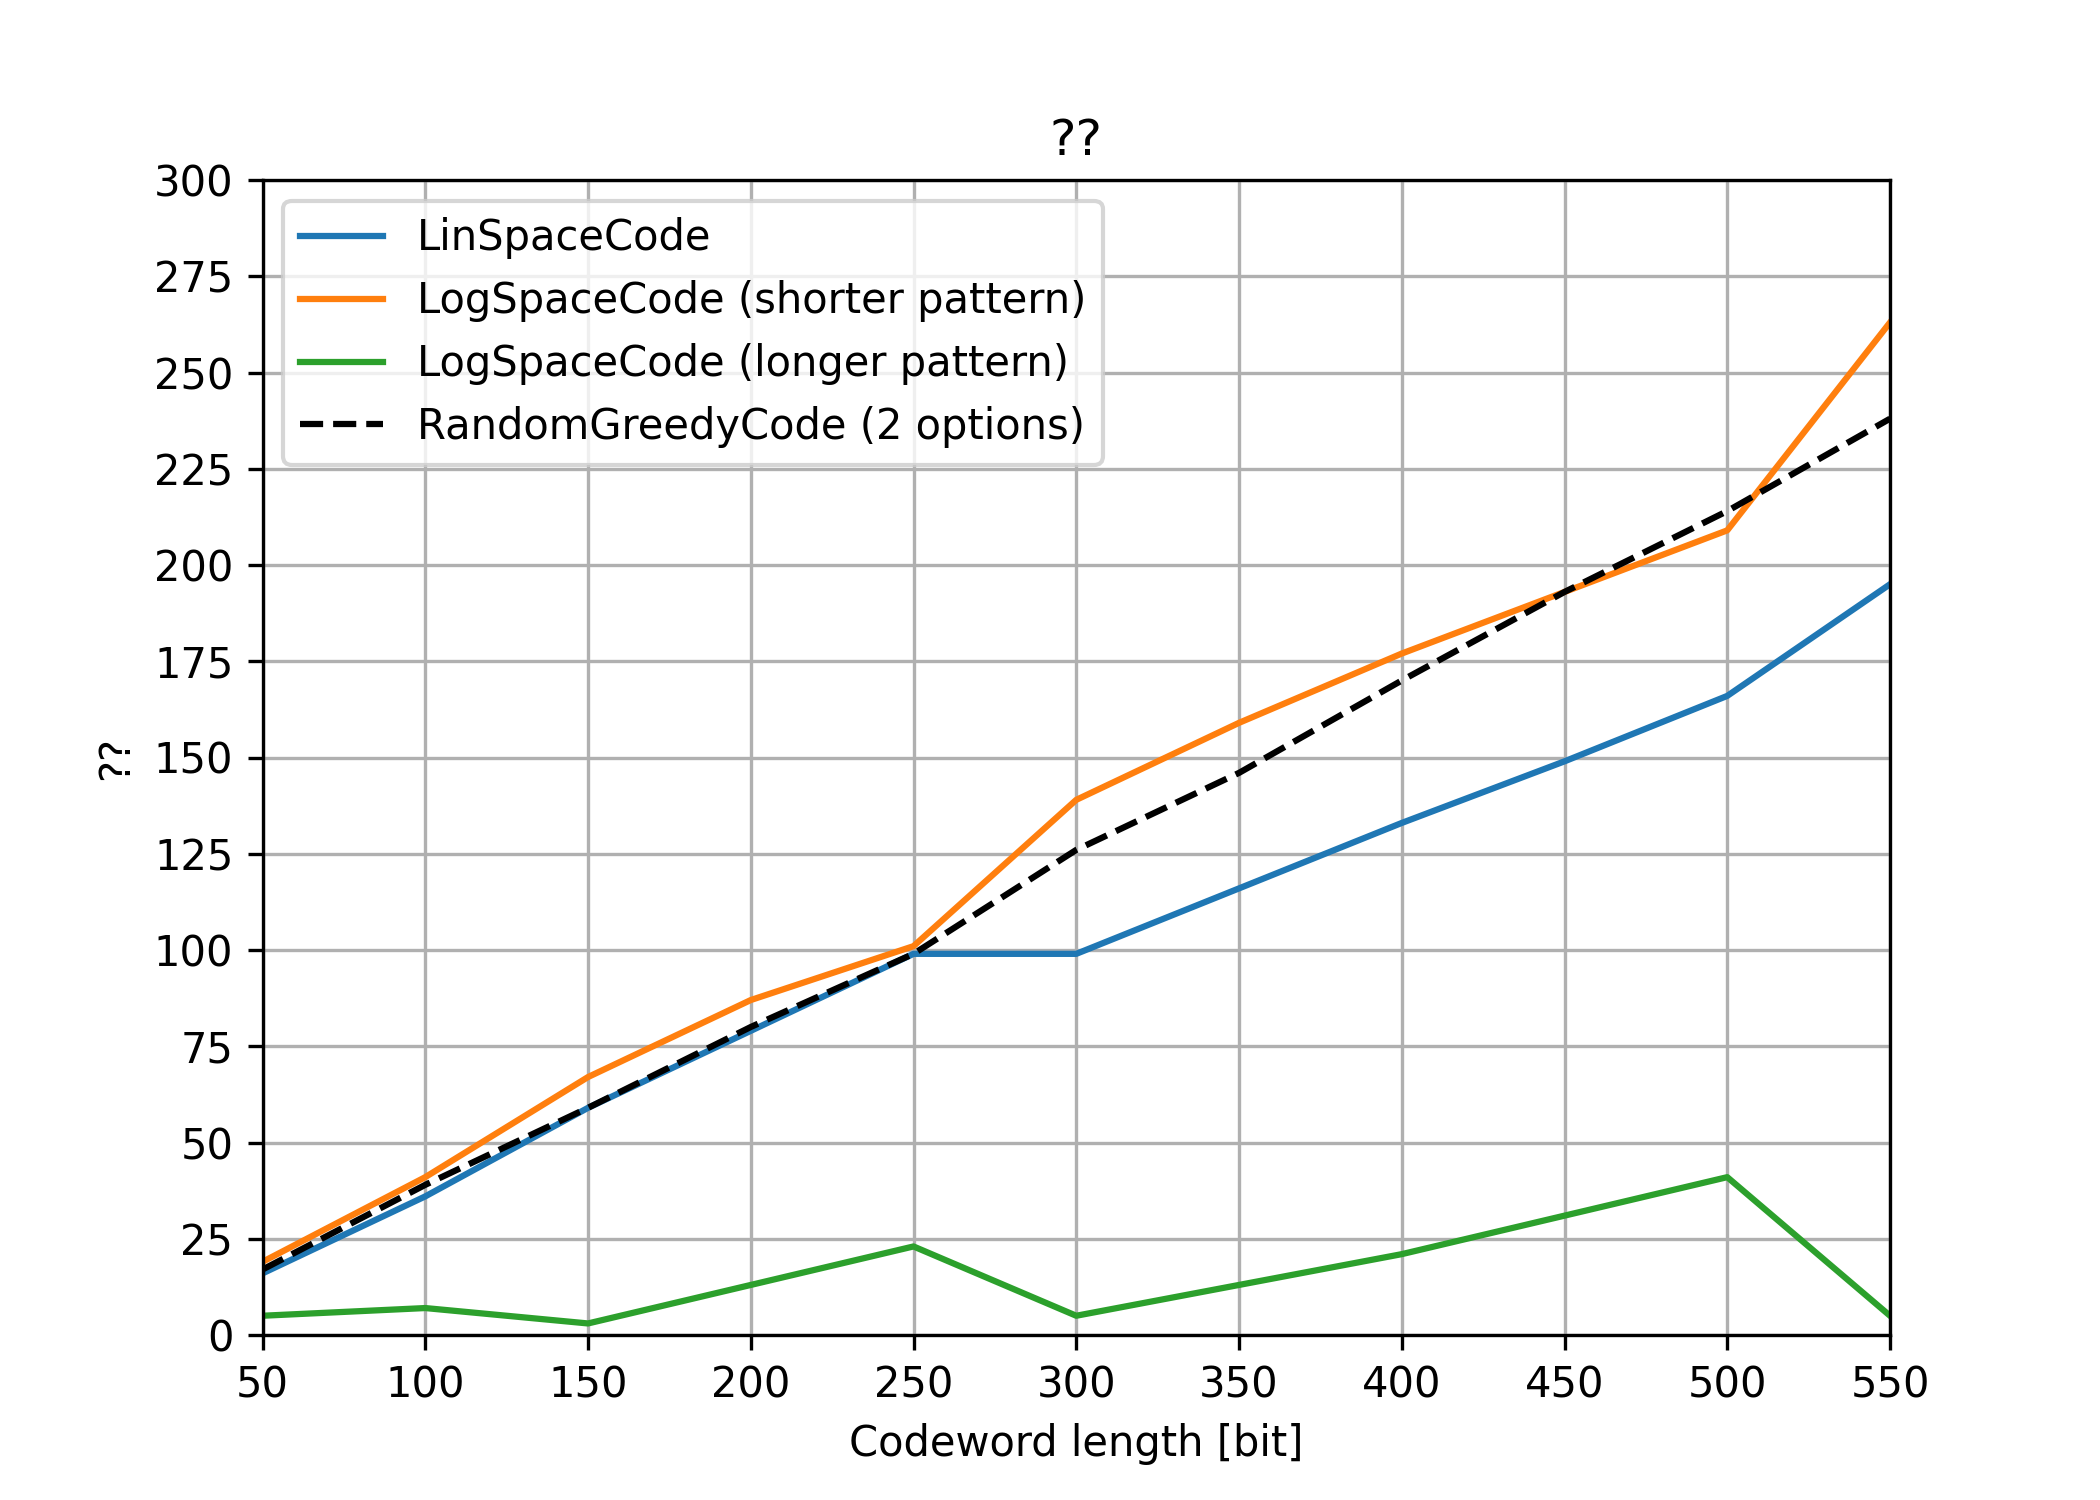
\includegraphics[width=1\textwidth]{artifacts/figure2.png}
    \caption{Comparison between the linspace and logspace codes.}
\end{figure}

\noindent In Figure 2, we see that the logspace code is slightly better than the linspace one. However, their results are comparable to the random/greedy code which has a far greater number of words. Therefore, the lower number of codewords in these codes does not seem to pay off.

\begin{figure}[H]
    \centering
    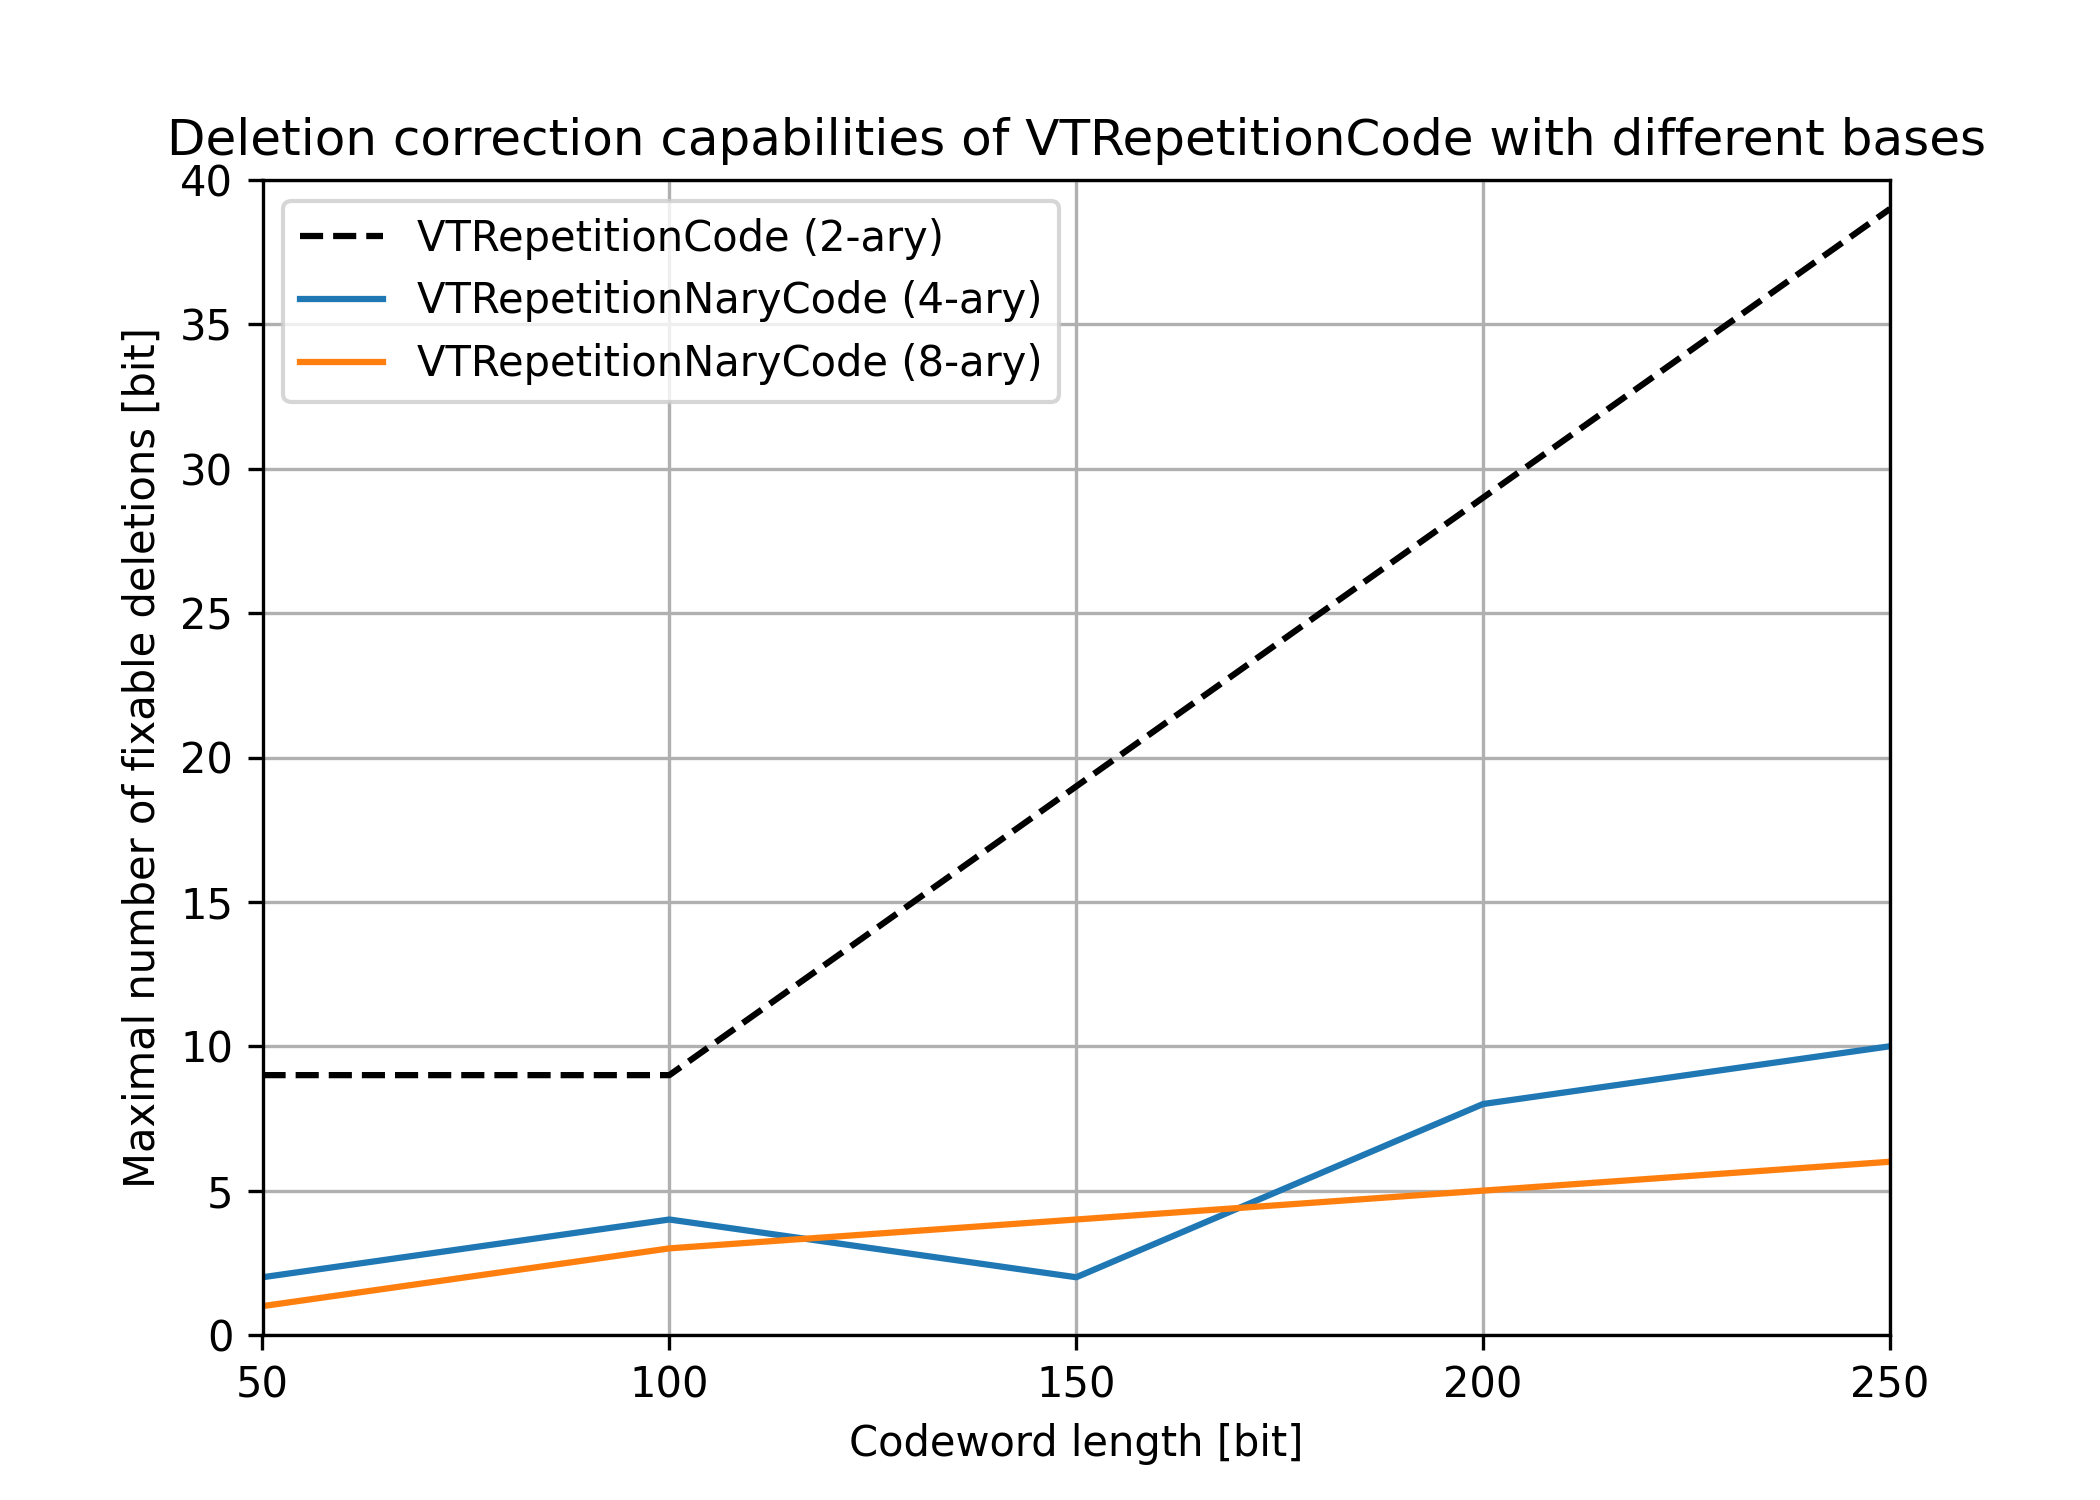
\includegraphics[width=1\textwidth]{artifacts/figure3.png}
    \caption{Comparison between the n-ary code with different bases.}
\end{figure}

\noindent Next, we tried generating the n-ary code with bases other than 4 (and 2, if we include the binary version). In Figure 3 we see that a higher base gives worse results. Base 8 was generally worse than base 4, which was itself worse than the binary code.

\begin{figure}[H]
    \centering
    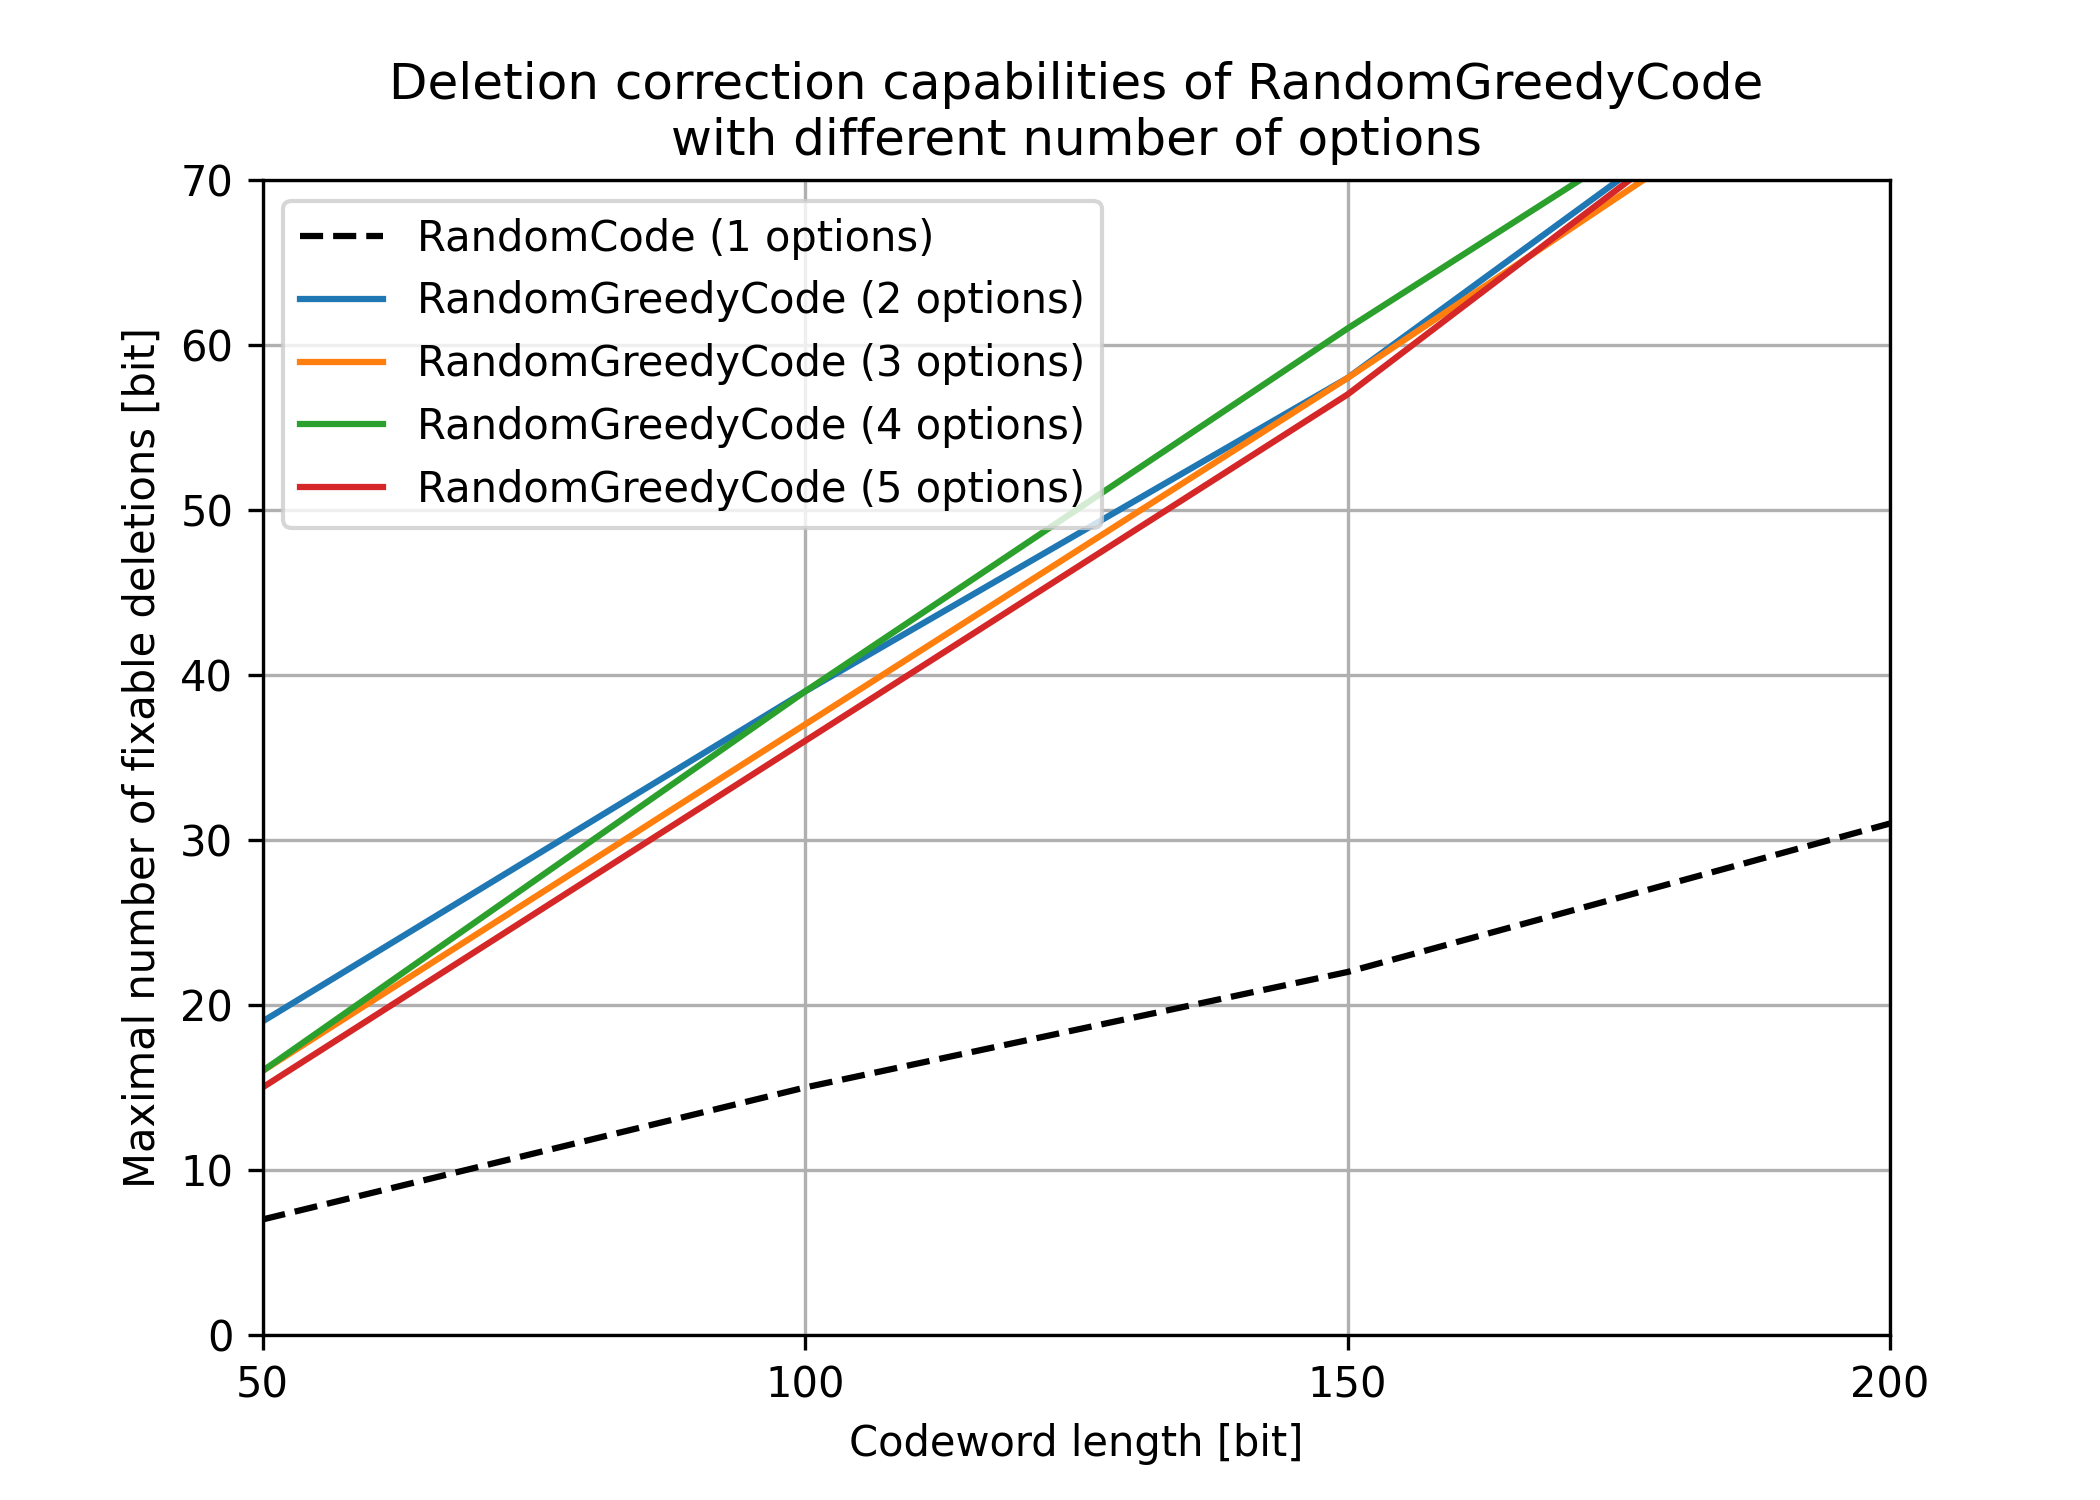
\includegraphics[width=1\textwidth]{artifacts/figure4.png}
    \caption{Comparison between the random/greedy code with a different number of codeword candidates.}
\end{figure}

\noindent Lastly, since the random/greedy code seemed to work so well, we thought to try and modify it. Instead of generating a pair of words in each iteration, we generate a number of words, which is equal to the parameter 'options'. For example, if options=3 we generate three words in each iteration and add the best one of those three to the code. Figure 4 displays the performance of the random/greedy code when generated with different values of the 'options' parameter. As we see in the figure, increasing the parameter of codeword candidates does not affect the possible number of corrections (but it does increase the time it takes to generate the code). Therefore, our original choice of 'options' to be 2 was sufficient.

In conclusion, the main takeaway from this project is the random/greedy code. It might be worth checking how this idea can be expanded to give even better deletion-correction capabilities.

\clearpage
\bibliographystyle{plain}
\bibliography{report/bibliography.bib}

\end{document}
